\documentclass{article}[18pt]
\usepackage{../../../../format}
\lhead{Networks and Systems - Networks}


\begin{document}
\begin{center}
\underline{\huge Wireless MAC}
\end{center}
\section{Elements of a wireless network}
Wireless hosts:
\begin{itemize}
	\item Laptop, smartphone
	\item Run applications
	\item May be stationary or mobile
\end{itemize}
Base station:
\begin{itemize}
	\item Typically connected to wired network
	\item Relay - responsible for sending packets between wired network and wireless host(s) in its "area" 
\end{itemize}
Wireless link:
\begin{itemize}
	\item Typically used to connect mobile(s) to base station
	\item Also used as backbone link
	\item Multiple access protocol coordinates link access
	\item Various data rates, transmission distances
\end{itemize}
Infrastructure mode:
\begin{itemize}
	\item Base station connects mobiles into wired network
	\item Handoff: mobile changes base station providing connection into wired network
\end{itemize}
Ad hoc mode:
\begin{itemize}
	\item No base stations
	\item Nodes can only transmit to other nodes within link coverage
	\item Nodes organize themselves into a network: route among themselves
\end{itemize}
\begin{tabular}{|c|c|c|}
	\hline 
	Standard & Frequency Range & Data Rate \\ 
	\hline 
	802.11b & 2.4 GHz & Up to 11 Mbps \\ 
	\hline 
	802.11a & 5 GHz & Up to 54 Mbps \\ 
	\hline 
	802.11g & 2.4 GHz & Up to 54 Mbps \\ 
	\hline 
	802.11n & 2.4 GHz and 5 GHz & Up to 450 Mbps \\ 
	\hline 
	802.11ac & 5GHz & Up to 1300 Mbps \\ 
	\hline 
\end{tabular} 
\section{Wireless Link Characteristics}
Important differences from wired link
\begin{itemize}
	\item Decreased signal strength: radio signal attenuates as it propagates through matter
	\item Interference from other sources: standardized wireless network frequencies shared by other devices interfere as well
	\item Multipath propagation: radio signal reflects off object ground, arriving at destination at slightly different times
\end{itemize}
Make communication across a wireless link much more difficult
\begin{defin}[Hidden terminals]
Senders that cannot sense each other but nonetheless collide at intended receiver
\end{defin}
Multiple wireless senders and receivers create additional problems (beyond multiple access)\\
\begin{minipage}{0.5\textwidth}
\includegraphics[scale=0.7]{"hidden terminal"}\\
Hidden terminal problem
\begin{itemize}
	\item B,A hear each other
	\item B,C hear each other
	\item A,C can't hear each other, means A,C unaware of their interference at B 
\end{itemize}
\end{minipage}
\begin{minipage}{0.5\textwidth}
\includegraphics[scale=0.7]{"signal attenuation"}\\
Signal attenuation:
\begin{itemize}
	\item B,A hear each other
	\item B,C hear each other
	\item A,C can't hear each other interfering at B
\end{itemize}
\end{minipage}
\begin{defin}[Exposed terminals]
Senders who can sense each other but still transmit safely (to different receivers)
\end{defin}
\section{802.11 LAN architecture}
Wireless host communicates with base station:
\begin{itemize}
	\item Base station = access point (AP)
\end{itemize}
Basic Service Set (BSS) (aka "cell") in infrastructure mode contains:
\begin{itemize}
	\item Wireless hosts
	\item Access point (AP): base station
	\item Ad hoc mode: hosts only
\end{itemize}
\section{802.11: Channels, association}
802.11b: 2.4 GHz - 2.485 GHz spectrum divided into 11 channels at different frequencies
\begin{itemize}
	\item AP admin chooses frequency for AP
	\item Interference possible: channel can be same as that chosen by neighbouring AP 
\end{itemize}
Host must associate with an AP
\begin{itemize}
	\item Scans channels, listening for beacon frames containing AP's name (SSID) and MAC address
	\item Selects AP to associate with
	\item May perform authentication
\end{itemize}
\section{802.11: passive/active scanning}
\begin{minipage}{0.5\textwidth}
\includegraphics[scale=0.7]{"passive scanning"}
Passive scanning
\begin{enumerate}
	\item Beacon frames sent from APs
	\item Association request frame sent: H1 to selected AP
	\item Association response frame sent from selected AP to H1
\end{enumerate}
\end{minipage}
\begin{minipage}{0.5\textwidth}
\includegraphics[scale=0.7]{"active scanning"}
Active scanning
\begin{enumerate}
	\item Probe request frame broadcast from H1
	\item Probe response frames sent from APs
	\item Association request frame sent: H1 to selected AP
	\item Association response frame sent from selected AP to H1
\end{enumerate}
\end{minipage}
\section{802.11: multiple access}
\begin{itemize}
	\item Avoid collisions: 2+ nodes transmitting at same time
	\item 802.11: CSMA - sense before transmitting - don't collide with ongoing transmission by another node
	\item 802.11: no collision detection
	\begin{itemize}
		\item Difficult to receive (sense collisions) when transmitting due to weak received signals (fading)
		\item Can't sense all collisions in any case: hidden terming, fading
		\item Goal: avoid collisions: CSMA/CA
	\end{itemize}
\end{itemize}
\section{IEEE 802.11 MAC Protocol: CSMA/CA}
802.11 sender
\begin{enumerate}
	\item If sense channel idle for DIFS then transmit entire frame (no CD)
	\item If sense channel busy then
	\begin{itemize}
		\item Start random backoff time
		\item Timer counts down while channel idle
		\item Transmit when timer expires
		\item If no ACK, increase random backoff interval, repeat 2
	\end{itemize}
\end{enumerate}
802.11 receiver
\begin{itemize}
	\item If frame received OK return ACK after SIFS (ACK needed due to hidden terminal problem)
\end{itemize}
Idea: allow sender to "reserve" channel rather than random access of data frames: avoid collisions of long data frames
\begin{itemize}
	\item Sender first transmits small request-to-send (RTS) packets to BS using CSMA
	\begin{itemize}
		\item RTSs may still collide with each other (but they're short)
	\end{itemize}
	\item BS broadcasts clear-to-send CTS in response to RTS
	\item CTS heard by all nodes
	\begin{itemize}
		\item Sender transmits data frame
		\item Other stations defer transmissions
	\end{itemize}
\end{itemize}
\begin{important}[Collisions]
Avoid data frame collisions completely using small reservations packets
\end{important}
\section{802.11 frame: addressing}
\begin{center}
	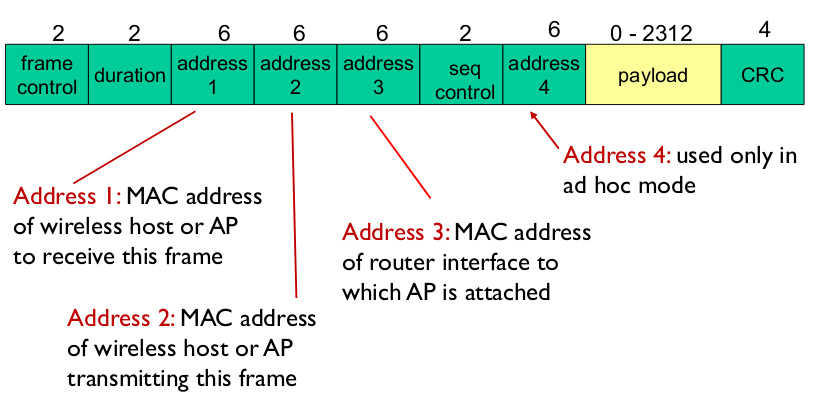
\includegraphics[scale=0.7]{addressing}
\end{center}
\begin{center}
	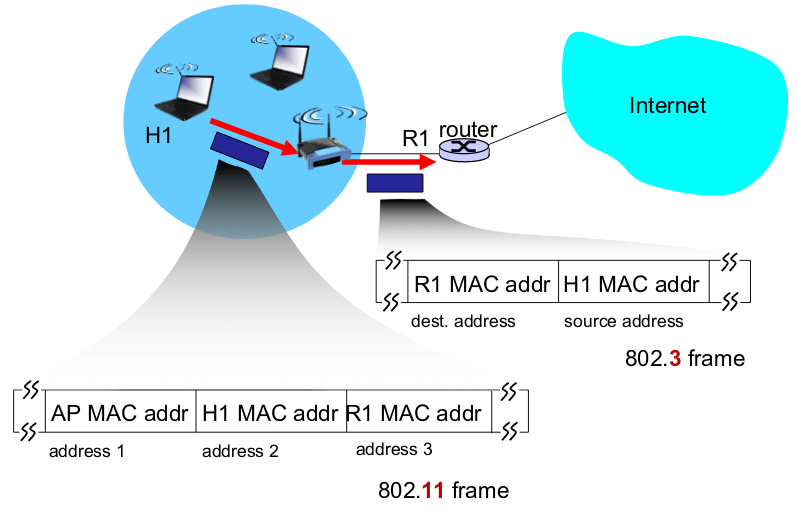
\includegraphics[scale=0.7]{addressing1}
\end{center}
\begin{center}
	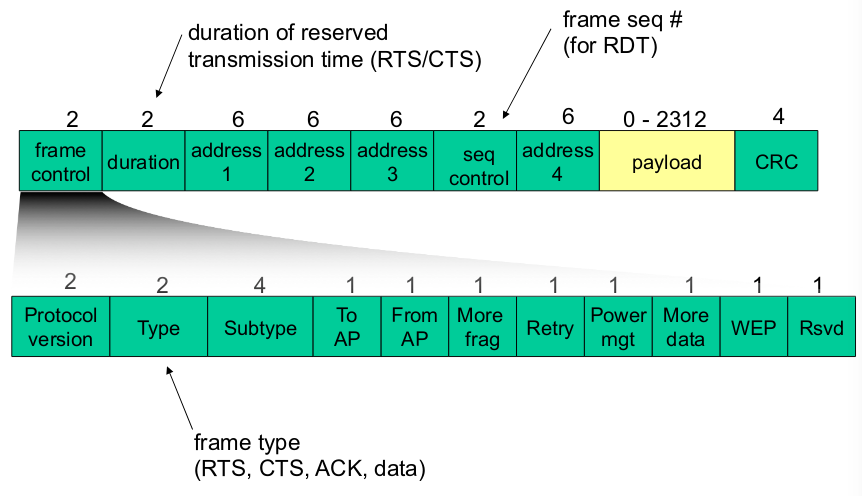
\includegraphics[scale=0.7]{addressing2}
\end{center}




\end{document}